\section {Assignment 6 \\ {Demosaicing Filter}}
\label {sec:assignment_6}

\subsection{Write C/C++ code for capturing a raw image}

\begin{lstlisting}[language=C, caption=save image to file, label=lst:rawcode]
// capture raw image
imshow(camName, image);
if (captRAW == true) {
    captRAW = false;
    // save raw image
    cfg.camMode = CAM_MODE_RAW;
    cam0.captureFrame(&image);
    imwrite("../capt/RAW.png", image);

    // save color image
    cfg.camMode = CAM_MODE_COL;
    cam0.captureFrame(&image);
    imwrite("../capt/COL.png", image);
}
\end{lstlisting}

the output of the code is shown in figure \ref{fig:input}.

\begin{figure}[ht]
    \centering
    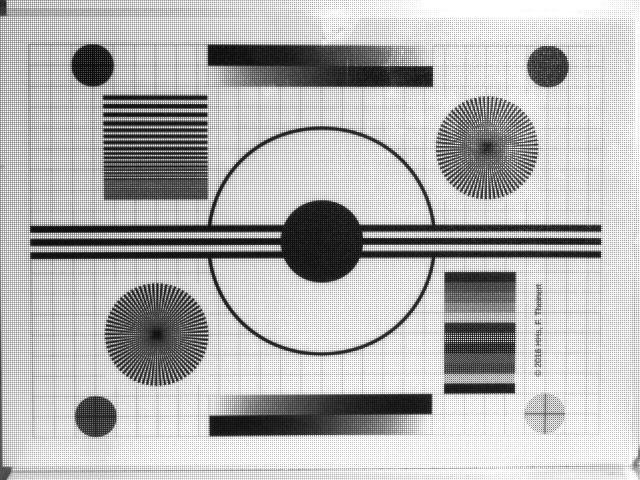
\includegraphics[width=0.5\textwidth]{test_RAW.png}
    \caption{test image}
    \label{fig:input}
    \end{figure}

\subsection{Convert this grayscale image to a color image by implementing a function to recover the actual colors}
The function prototype should look as follows:
\begin{lstlisting}[language=C, caption=function prototype, label=lst:prototype]
void deBayer(Mat *rawImg, Mat *outImg);
\end{lstlisting}


To convert the RAW image, we first splitt the image into 3 channels, one for each color. Then we interpolate the missing values in the channels. The result is a color image. The function for splitting is shown in listing \ref{lst:splitt}.

\begin{lstlisting}[language=C, caption=splitt image, label=lst:splitt]

for(row=0; row<rawImg->rows; row++){	//todo: make this evaluation smaller to increase speed
    for(col=0; col<rawImg->cols; col++){
        if (row % 2 == 0 && col % 2 == 0) //odd row, odd column
            outImgMID->at<Vec3b>(row, col).val[BGR_GREEN] = rawImg->at<uint8_t>(row,col);
        if (row % 2 == 0 && col % 2 == 1) //odd row, even column
            outImgMID->at<Vec3b>(row, col).val[BGR_RED] = rawImg->at<uint8_t>(row,col);
        if (row % 2 == 1 && col % 2 == 0) //even row, odd column
            outImgMID->at<Vec3b>(row, col).val[BGR_BLUE] = rawImg->at<uint8_t>(row,col);
        if (row % 2 == 1 && col % 2 == 1) //even row, even column
            outImgMID->at<Vec3b>(row, col).val[BGR_GREEN] = rawImg->at<uint8_t>(row,col);			
    }
}

\end{lstlisting}

And the function for interpolating is shown in listing \ref{lst:interpolate}, ware as a exaple the green channel is interpolated.
This function interpolates the missing values in the channels, by using the values of the neighboring pixels. The result is a color image.

\begin{lstlisting}[language=C, caption=interpolate missing values, label=lst:interpolate]

// Interpolate green channel by taking the value of the nearest neighbour that is green
std::cout << "Interpolating green channel" << std::endl;

for(row=0; row<outImgMID->rows; row++){
    for(col=0; col<outImgMID->cols; col++){
        if (outImgMID->at<Vec3b>(row, col).val[BGR_GREEN] == 0){
            if (col > 0 && outImgMID->at<Vec3b>(row, col-1).val[BGR_GREEN] != 0)
                outImg->at<Vec3b>(row, col).val[BGR_GREEN] = outImgMID->at<Vec3b>(row, col-1).val[BGR_GREEN];
            else if (col < outImgMID->cols-1 && outImgMID->at<Vec3b>(row, col+1).val[BGR_GREEN] != 0)
                outImg->at<Vec3b>(row, col).val[BGR_GREEN] = outImgMID->at<Vec3b>(row, col+1).val[BGR_GREEN];
            else if (row > 0 && outImgMID->at<Vec3b>(row-1, col).val[BGR_GREEN] != 0)
                outImg->at<Vec3b>(row, col).val[BGR_GREEN] = outImgMID->at<Vec3b>(row-1, col).val[BGR_GREEN];
            else if (row < outImgMID->rows-1 && outImgMID->at<Vec3b>(row+1, col).val[BGR_GREEN] != 0)
                outImg->at<Vec3b>(row, col).val[BGR_GREEN] = outImgMID->at<Vec3b>(row+1, col).val[BGR_GREEN];
        }
    }
}

\end{lstlisting}

This gives the output image shown in figure \ref{fig:output}. Which is different from the color image shown in figure \ref{fig:original}.
The difference between the original and the output, can be explained by an incorrect splitting of the image, or wrong interpolation.

\begin{figure}[ht]
\centering
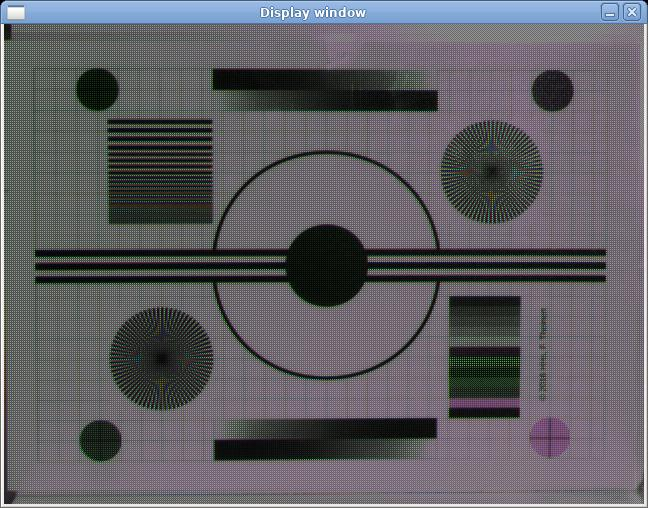
\includegraphics[width=0.5\textwidth]{out.png}
\caption{Output image}
\label{fig:output}
\end{figure}

\begin{figure}[ht]
\centering
\includegraphics[width=0.5\textwidth]{test_COL.png}
\caption{Original image}
\label{fig:original}
\end{figure}

For the full code see appendix \ref{sec:appendix_D}.